\section{Limits on a light CP-odd scalar}
For different values of the integrated luminosity, $95\%$ CL upper limits on the $t\bar{t}A$ production cross section times branching ratio, $\sigma(t\bar{t}A)\times {\rm BR}(A\to b\bar{b})$, as a function of $m_{A}$ (see figure \ref{sec:ttA:fig:limit}) are set using the CL$_{s}$ method. Those limits can be translated onto upper limits on $|g_{t}|$ assuming ${\rm BR}(A\to b\bar{b})=1$, as shown in table \ref{sec:ttA:tab:sigma_95CL}. 
This search can exclude a  CP-odd scalar that couples with $g_{t}=1$ for $20\le m_{A} \le90$ $\gev$ with 30 fb$^{-1}$ (the ATLAS detector in Run 2 has already collected 36.2 fb$^{-1}$ at $\sqrt{s}=13$ $\tev$); the scenario with 300 fb$^{-1}$ can exclude a coupling $g_{t}$ of order 0.5 in the mass range between 30 and 90 \gev. 

\begin{figure}[htbp!]
\begin{subfigure}{0.5\textwidth}
  \centering
  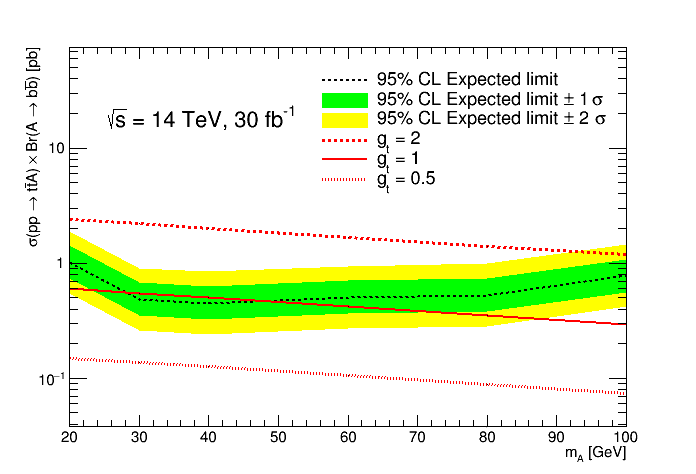
\includegraphics[width=0.9\textwidth]{figures/ttA/limit_30fb.png}
  \caption{}
  \label{}
\end{subfigure}
\begin{subfigure}{0.5\textwidth}
  \centering
  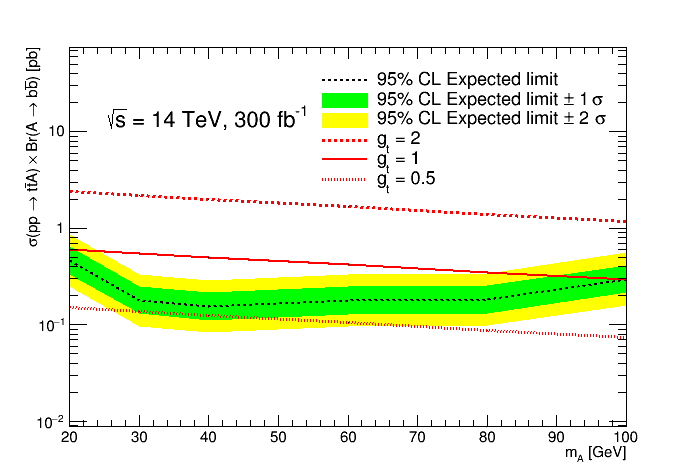
\includegraphics[width=0.9\textwidth]{figures/ttA/limit_300fb.png}
  \caption{}
  \label{}
\end{subfigure}
\captionsetup{width=0.85\textwidth} \caption{\small Expected $95\%$ CL upper limits on $\sigma(t\bar{t}A)\times {\rm BR}(A\to b\bar{b})$ as a function of $m_{A}$  in $pp$ collisions at $\sqrt{s}$= 14 $\tev$ for an integrated luminosity of (a) 30 fb$^{-1}$ and (b) 300 fb$^{-1}$.  The green and yellow bands correspond to 1 and 2 standard deviations respectively around the median expected limit under the background-only hypothesis.  Also shown are the theoretical cross sections for $\sigma(t\bar{t}A)$ for different assumed values of $g_{t}$ (0.5, 1.0, and 2.0) and ${\rm BR}(A\to b \bar{b})=1$.}
\label{sec:ttA:fig:limit}
\end{figure}


\begin{table}[htb!]\footnotesize
\begin{center} 
\begin{tabular}{ccccccc} 
\hline\hline
 & \multicolumn{6}{c}{95\% CL upper limits on $\sigma(t\bar{t} A) \times {\rm BR}(A\to b\bar{b})$ (pb)} \\
\hline
  & \multicolumn{6}{c}{$m_A$ (GeV)} \\
  \cline{2-7} 
${\cal L}$ (fb$^{-1}$) & $\quad$ 20 $\quad$ & $\quad$ 30 $\quad$ & $\quad$ 40 $\quad$ & $\quad$ 60 $\quad$ & $\quad$ 80 $\quad$ & $\quad$ 100 $\quad$ \\
\hline
30 & 1.02 & 0.48 & 0.45 & 0.51 & 0.53 & 0.78  \\
300 & 0.46 & 0.18 & 0.16 & 0.18 & 0.18 & 0.30 \\
3000 & 0.17 & 0.066 & 0.057 & 0.065 & 0.065 & 0.13 \\
\hline\hline
\end{tabular} 
\captionsetup{width=0.85\textwidth} \caption{\small Expected 95\% CL upper limits on $\sigma(t\bar{t} A) \times {\rm BR}(A\to b\bar{b})$ as a function of $m_A$ in $pp$ collisions at $\sqrt{s}=14$ TeV for different integrated luminosities.}
\label{sec:ttA:tab:sigma_95CL} 
\end{center} 
\end{table} 


\subsection{Interpretation of the limits}

A light CP-odd Higgs boson ($m_{A}<125$ $\gev$), which may or may not be related to global symmetries being present, exists in many extensions of the SM. This search is interpreted in several representative BSM scenarios. 

In the context of Type-I and Type-II 2HDM models, the $g_{t\bar{t}A}$ coupling is $\cot\beta$ enhanced and it can cover regions with $\tan\beta<5$. The limits in the $m_{A}$ vs. $\tan\beta$ plane are presented for this search and for a search that targets $b\bar{b}A$ production \cite{Kozaczuk:2015bea} in figure \ref{sec:ttA:fig:2hdm}. For a Type-I 2HDM, where both couplings are $\cot\beta$ enhanced, the $t\bar{t}A$ has a better sensitivity. Instead, for a Type-II 2HDM  the $g_{b\bar{b}A}$ coupling is $\tan\beta$ enhanced and it leads to a complementarity of the two analysis on the plane, which can cover the whole parameter region except a corner with relatively large $m_{A}$ and moderate $\tan\beta$. As shown in figure \ref{sec:ttA:fig:2hdm} the green region of the plane, which can explain the gamma-ray excess in the Galactic Centre, can be effectively probed by the proposed $t\bar{t}A$ search.


\begin{figure}[htb!]
\centering
\begin{subfigure}{0.45\textwidth}
  \centering
  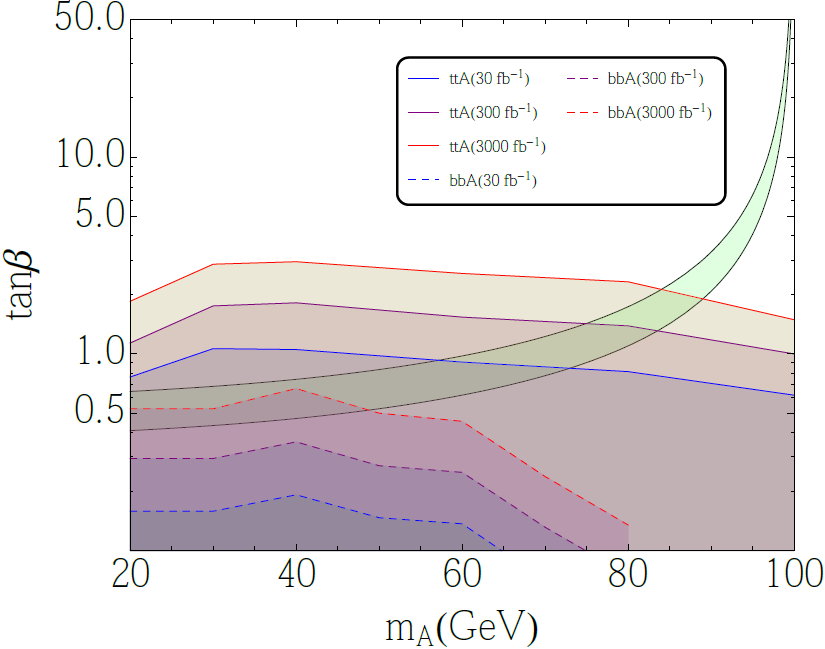
\includegraphics[width=0.9\textwidth]{figures/ttA/fig7a.png}
  \caption{}
  \label{}
\end{subfigure}
\begin{subfigure}{0.45\textwidth}
  \centering
  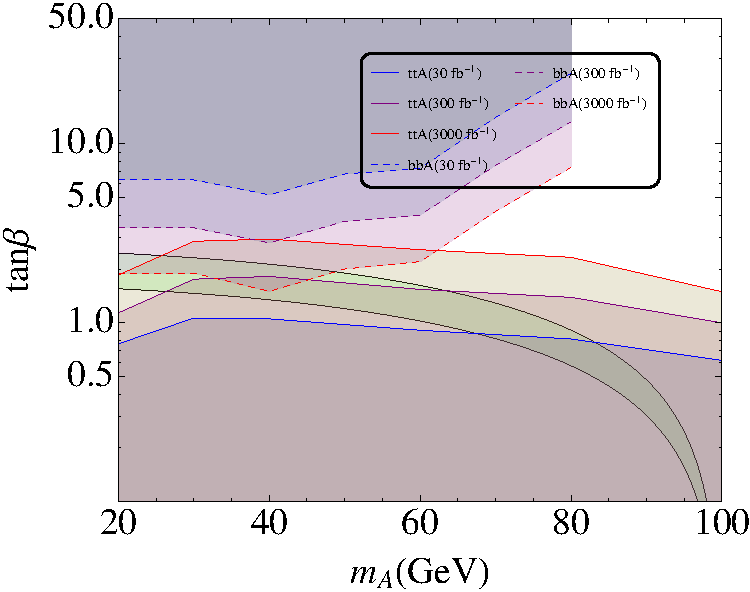
\includegraphics[width=0.9\textwidth]{figures/ttA/fig7b.png}
  \caption{}
  \label{}
\end{subfigure}
\captionsetup{width=0.85\textwidth} \caption{\small Sensitivity reach (at $95\%$ CL) of the $b\bar{b}A$ and  $t\bar{t}A$ channels within the (a) Type-I 2HDM and (b) Type-II 2HDM. The green bands represent a region where the recently observed gamma-ray excess from the Galactic Centre can be explained.}
\label{sec:ttA:fig:2hdm}
\end{figure}

In the context of the NMSSM in the R-limit \cite{Espinosa:1992sk} and in the PQ-limit \cite{Schuster:2005py} this $t\bar{t}A$ search has very little sensitivity even at luminosity of 3 ab$^{-1}$, as shown in figure \ref{sec:ttA:fig:nmssm}.


\begin{figure}[htb!]
\centering
\begin{subfigure}{0.45\textwidth}
  \centering
  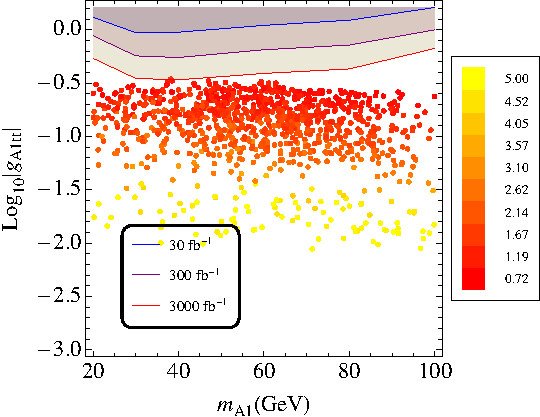
\includegraphics[width=0.9\textwidth]{figures/ttA/fig8a.png}
  \caption{}
  \label{}
\end{subfigure}
\begin{subfigure}{0.45\textwidth}
  \centering
  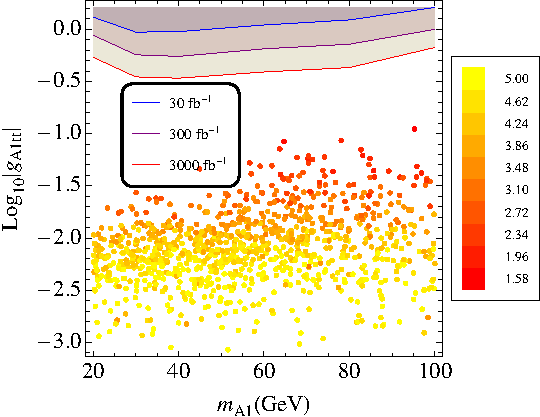
\includegraphics[width=0.9\textwidth]{figures/ttA/fig9a.png}
  \caption{}
  \label{}
\end{subfigure}
\captionsetup{width=0.85\textwidth} \caption{\small Sensitivity reach (at $95\%$ CL) to the (a) R-limit and (b) PQ-limit scenarios in the NMSSM via the $t\bar{t}A$. The hue of the scatter points represents the corresponding $\tan\beta$ values. }
\label{sec:ttA:fig:nmssm}
\end{figure}